
\documentclass{beamer}
\usetheme{Goettingen}
\usepackage{hyperref}
\begin{document}
%\nocite{voss2007essentials}
\title{Chapter 8: Maps and related tasks}  
\author{Harm Dubois \and Joris Stork}
\date{\today} 

\frame{\titlepage} 
\section{Blah} 
\frame{\tableofcontents} 

\section{Blah} 

\subsection{Blah} 
\frame{\frametitle{Blah}
}

\subsection{Blah} 
\frame{\frametitle{Blah}
}

\subsection{Blah}
\frame{\frametitle{Blah}
\begin{columns}[c]
\column{5cm}
\begin{quote}
``[...] the essential, domain-independent skills
necessary for acquiring a wide range of domain-specific [...] data \&
skills - i.e. the ability to learn anything (in principle). More specifically,
this learning ability needs to be autonomous, goal-directed, and highly
adaptive'' \em{- Peter Voss, 2007: \cite{voss2007essentials}}
\end{quote}
\column{5cm}
% 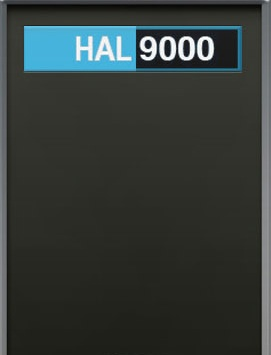
\includegraphics[width=5cm]{halsub1}
\end{columns}
}
\end{document}
